\author{Patrick Bucher}
\title{px: PEAX Command Line Client}
\subtitle{Wirtschaftsprojekt, Herbstsemester 2019}
\date{\today}
\maketitle
\thispagestyle{empty}

\section*{Abstract}

Die Software \texttt{px} ist ein Kommandozeilenprogramm, das den Zugriff auf die RESTful-API von PEAX für Benutzer mit einem technischen Hintergrund vereinfachen soll. PEAX ist ein digitaler Briefkasten, womit Endanwender ihre Post über verschiedene Kanäle empfangen und in einem komfortablen Web-Portal verwalten können. Mit \texttt{px} soll der direkte Zugriff auf die RESTful API, d.h. ohne Verwendung des Webportals, vereinfacht werden, indem die Handhabung von Tokens (Access Token, Refresh Token) abstrahiert wird, und dem Benutzer intuitiv bedienbare sowie generische (d.h. HTTP-nahe) Befehle für das Ansteuern verschiedener Endpoints zur Verfügung gestellt werden.

\vfill

\begin{center}
    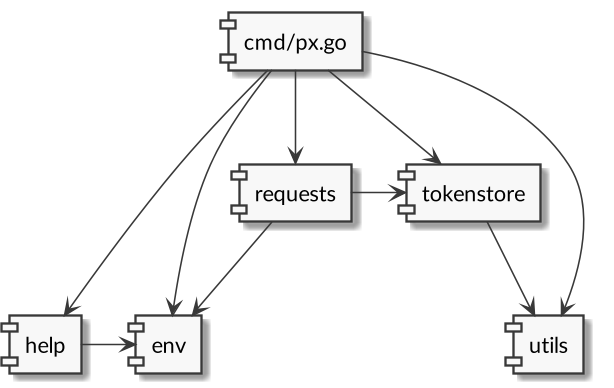
\includegraphics[width=0.7\linewidth]{pics/title.png}
\end{center}
